A perturbációszámítás a Green-függvény egyik legjelentősebb alkalmazása. Ebben a részben a Green-függvény perturációs sorának a konvergencia tulajdonságait vizsgáljuk. A konvergencia tartományát és sebességét befolyásolja a perturbáló operátor triviális módosítása, konkrétan a vizsgált példában az $\frac{FL}{2}\op{I}$ operátort a perturbáló tagból levonjuk és a perturálatlan operátorhoz hozzáadjuk. Ezzel a teljes Hamilton operátor nem változik, de a perturbációs sor konvergenciája igen.

A perturbációszámításhoz a Hamilton operátort két részre bontjuk,
\begin{equation}
	\op{H} = \op{H}_0 + \op{V}.
\end{equation}
A $\op{H}_0$ operátorhoz tartozó rezolvens operátor $\op{G}_0\left(E\right)$. Mind $\op{H}$ és mind $\op{H}_0$ kifejezhetőek a rezolvenseikkel, ha ezeket behelyettesítjük a fenti egyenletbe, implicit egyenletet kapunk $\op{G}\left(E\right)$-re nézve,
\begin{equation}
	-\op{G}^{-1}\left(E\right) - E = -\op{G}_0^{-1}\left(E\right) - E + \op{V}.
\end{equation}
Ezt kisebb átalakítások után fel lehet használni perturbációszámításra. Az egyenletet balról $\op{G}_0\left(E\right)$-vel, jobbról $\op{G}\left(E\right)$-vel szorozzuk, így
\begin{equation}
	\op{G}\left(E\right) = \op{G}_0\left(E\right) + \op{G}_0\left(E\right)\op{V}\op{G}\left(E\right)
	\label{green:pertmaster}
\end{equation}
eredményhez jutunk. Megfelelően definiálva $\op{G}_n\left(E\right)$ operátorokat,
\begin{equation}
	\op{G}_n\left(E\right) = \op{G}_0\left(E\right)\sum_{k=0}^n\left(\op{V}\op{G}_0\left(E\right)\right)^k,
\end{equation}
\aeqref{green:pertmaster} egyenlethez hasonló rekurziós összefüggés áll fent,
\begin{equation}
	\op{G}_{n+1}\left(E\right) = \op{G}_0\left(E\right) + \op{G}_0\left(E\right)\op{V}\op{G}_n\left(E\right).
	\label{perturbation:rekurzió}
\end{equation}
Ha $\norm{\op{V}\op{G}_0\left(E\right)} < 1$ akkor a $\op{G}_n$ sorozat konvergál. A sor határértéke \aeqref{perturbation:rekurzió} miatt kielégíti \aeqref{green:pertmaster} egyenletet. Így konvergencia esetén
\begin{equation}
	\op{G}\left(E\right) = \op{G}_0\left(E\right)\sum_{n=0}^\infty\left(\op{V}\op{G}_0\left(E\right)\right)^n.
\end{equation}


A perturbálatlan operátornak a lineáris potenciál nélküli dobozba zárt részecske Hamilton operátorát választom, $\op{H}_0=\frac{1}{2m}\op{p}^2$, így a lineáris potenciál marad a perturbáció $\op{V} = F\op{x}$. A perturbálatlan $\op{G}_0\left(E\right)$ Green-függvényt is \aref{green:Cbegin}-\ref{green:Cend}, \ref{green:xy}. és \aref{green:yx}. egyenletek alapján határozom meg.
\begin{equation}
	G_0\left(x,y;E\right) = -\frac{2m}{k\hbar^2}\frac{1}{\sin\left(kL\right)}\times
	\begin{cases}
		\sin\left(k\left(y-L\right)\right)\sin\left(kx\right) & x\leq y\\
		\sin\left(k\left(x-L\right)\right)\sin\left(ky\right) & x\geq y\\
	\end{cases},
\end{equation}
\begin{equation}
	k = \frac{\sqrt{2mE}}{\hbar}.
\end{equation}
\begin{figure}[H]
	\centering
	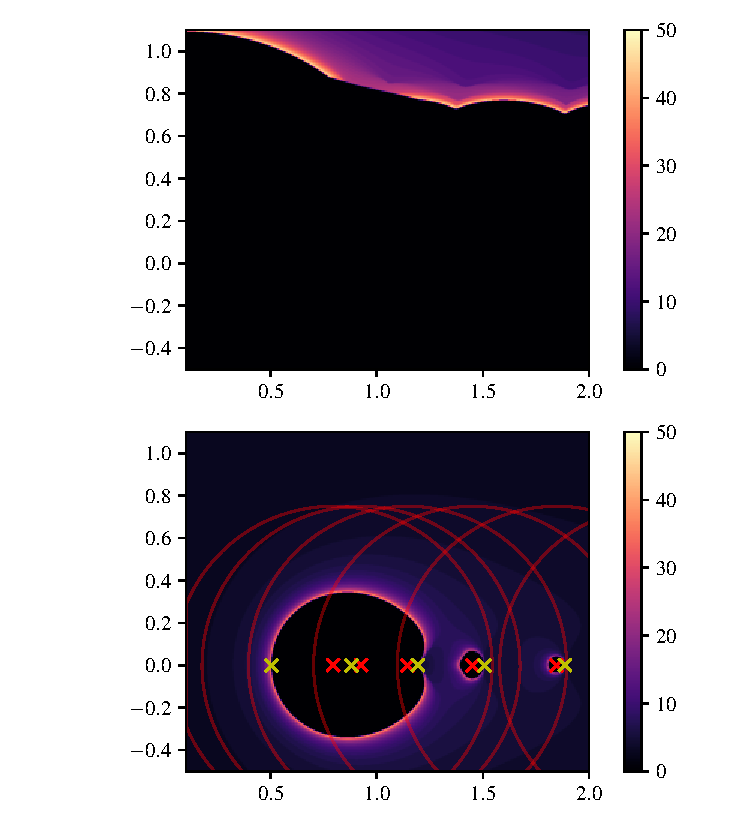
\includegraphics[scale=1]{./figs/convergence3.pdf}
	\caption[Green-függvény perturbációs sorának konvergenciája]{Ez az ábra a két perturbációs sor konvergenciáját hasonlítja össze a komplex energia síkon. A felső ábra a $V=Fx$ perturbáló potenciálnak, míg az alsó a $V = Fx-FL/2$ perturbáció szerinti sornak felel meg. A fekete tartományok divergenciát jelölnek, míg a többi szín a sorfejtés tagjainak csökkenési sebességét jellemzik, a norma harmadolásához szükséges lépések számát megadva. A piros körökön kívüli tartomány a ?? formula által garantált konvergencia tartományát jelöli. A piros x-ek a $\hat{G}_0$ pólusait, a sárga x-ek pedig az egzakt $\hat{G}$ operátor pólusait jelölik.}
\end{figure}